\documentclass[twocolumn]{article}
\usepackage[utf8]{inputenc}
\usepackage{graphicx}
\usepackage{tabularx}
\usepackage{subfigure}
\usepackage{hyperref}
\voffset = -100pt
\hoffset = -50pt
\headheight = 0pt
\textwidth = 550pt
\textheight = 750pt
\author{Name Surname }
\setlength{\columnsep}{0.3cm}
\usepackage{blindtext}
\pagestyle{empty}
\footskip = 0pt
\bibliographystyle{plain}

\begin{document}

\section*{Viktor Pavlov 230335TAF}
\section{Music Genre Classification via MFCC Analysis}
\begin{figure}[htbp]
  \centering
  \begin{minipage}[t]{0.5\columnwidth}
    \centering
    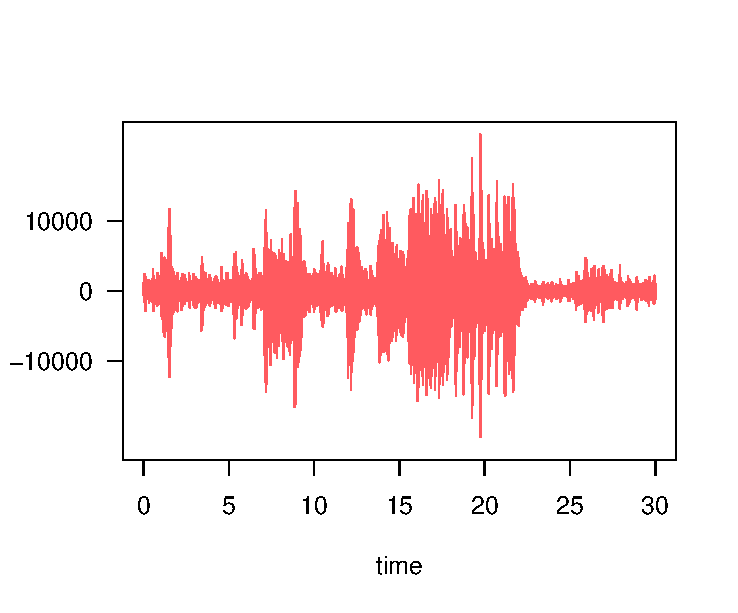
\includegraphics[width=\linewidth]{images/audio_jazz.pdf}
  \end{minipage}\hfill
  \begin{minipage}[t]{0.5\columnwidth}
    \centering
    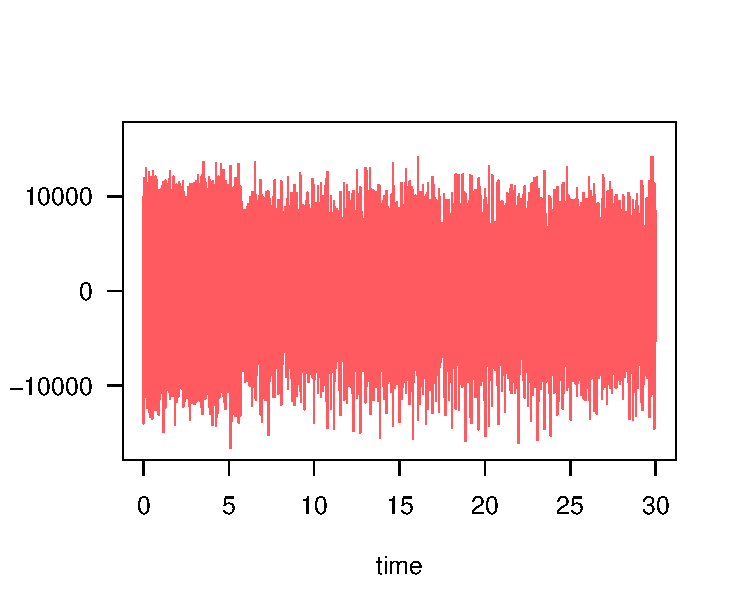
\includegraphics[width=\linewidth]{images/audio_metal.pdf}
  \end{minipage}
  \caption{Continuation (right) generated by the Unconditional Transformer model based on primer (left).}
  \label{fig:groupedImages}
\end{figure}
\blindtext

\section{MFCC Audio Feature Extraction}

\blindtext

\section{K-Means Clustering}
\begin{figure}[hht]
\centering
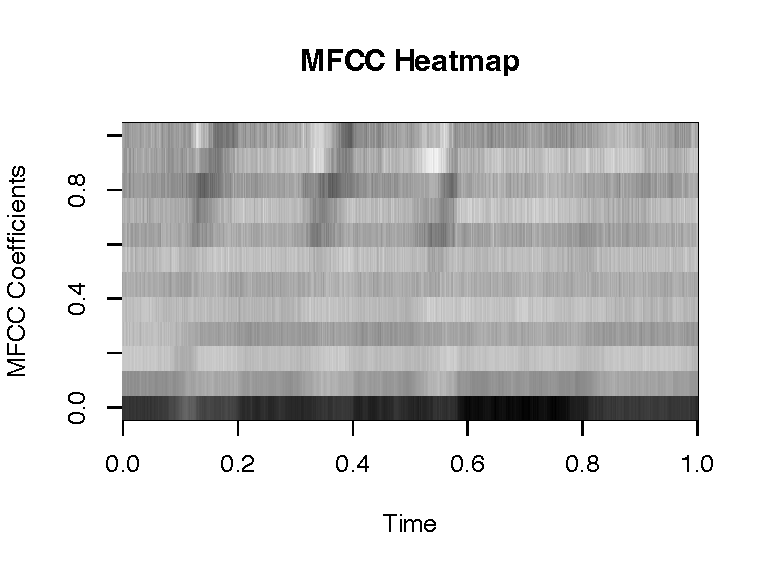
\includegraphics[width=0.49\textwidth]{images/mfcc_heatmap_8.pdf}
\caption{Correlation heat map of the Boston Housing dataset.}
\label{fig:corr}
\end{figure}


\blindtext

\section{Classification using Support Vector Machines (SVM)}
\begin{figure}[hht]
	\centering
	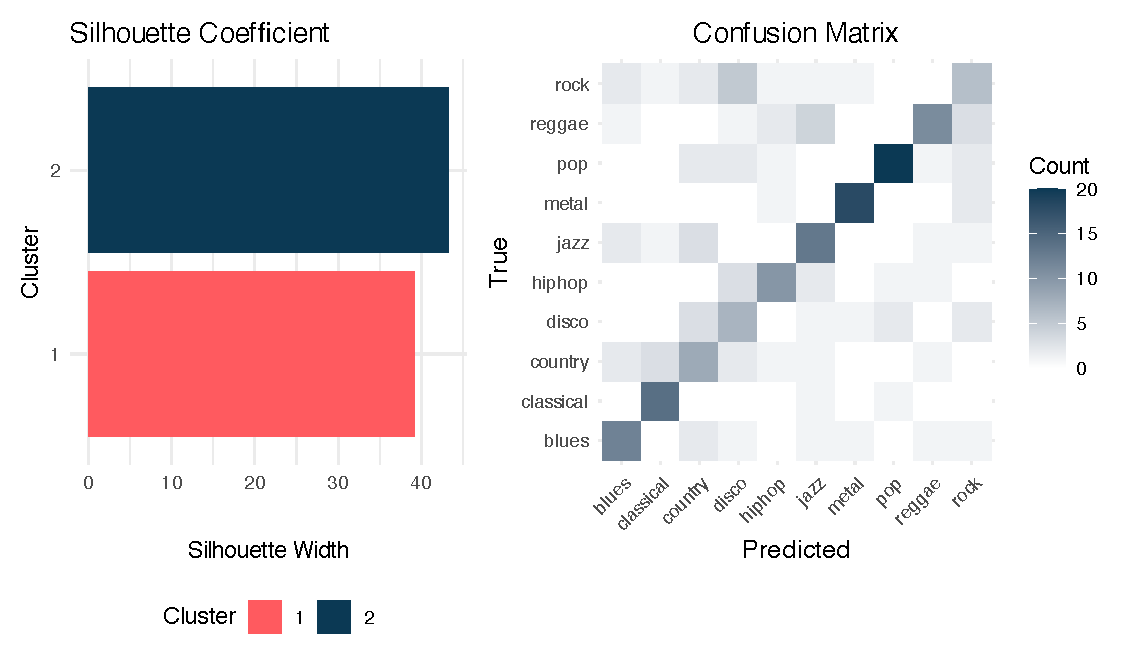
\includegraphics[width=0.49\textwidth]{images/clust_class.pdf}
  \caption{Correlation heat map of the Boston Housing dataset.}
	\label{fig:corr}
\end{figure}

\blindtext

\bibliography{bibliography}

\end{document}
